\capitulo{5}{Aspectos relevantes del desarrollo del proyecto}

%Este apartado pretende recoger los aspectos más interesantes del desarrollo del proyecto, comentados por los autores del mismo.
%Debe incluir desde la exposición del ciclo de vida utilizado, hasta los detalles de mayor relevancia de las fases de análisis, diseño e implementación.
%Se busca que no sea una mera operación de copiar y pegar diagramas y extractos del código fuente, sino que realmente se justifiquen los caminos de solución que se han tomado, especialmente aquellos que no sean triviales.
%Puede ser el lugar más adecuado para documentar los aspectos más interesantes del diseño y de la implementación, con un mayor hincapié en aspectos tales como el tipo de arquitectura elegido, los índices de las tablas de la base de datos, normalización y desnormalización, distribución en ficheros3, reglas de negocio dentro de las bases de datos (EDVHV GH GDWRV DFWLYDV), aspectos de desarrollo relacionados con el WWW...
%Este apartado, debe convertirse en el resumen de la experiencia práctica del proyecto, y por sí mismo justifica que la memoria se convierta en un documento útil, fuente de referencia para los autores, los tutores y futuros alumnos.

%Despliegue continuo - direccion de app en heroku. Sistema gratuito sirve para validar, pero no para explotar
%Diseño extensible
%Framework vaadin
%No responsive

%Comparacion de tfgs en la ubu, captura dde pantalla con comparativa tfg
Este capítulo recoge los aspectos destacables durante el desarrollo del proyecto.
\section{Motivación de la elección}
La elección de este trabajo fue motivada por su relación con las asignaturas de la mención de ingeniería del software, detacando las asignaturas:\textit{Gestión de Proyectos}, \textit{Diseño y Mantenimiento del Software}, \textit{Desarrollo Avanzado de Sistemas Software}, en las que se enseña como desarrollar software de calidad usando repositorio Software.
\section{Evolución del proyecto}
Tras la elección del proyecto se acordó definir una evolución que siga las bases del modelo Scrum. Tomando un proceso de desarrollo incrementa con revisión de las iteraciones cada dos semanas.
Se han definido sprints de dos semanas. Estas reuniones constaban de dos partes:
\begin{itemize}
	\item Revisión del sprint: En las que se revisaba el incremento generado, los problemas que hubo durante su desarrollo, las soluciones que se han implementado o que se plantean para el siguiente sprint.
	\item Planificación del siguiente sprint: Se definían las nuevas tareas.
\end{itemize}
Las primeras fases del desarrollo fueron de investigación y configuración. Luego se planteó un diseño inicial, que fue la base para la implementación de nuevas funcionalidades aunque, con el tiempo, se fue modificando el diseño inicial para adaptarlo a las nuevas funcionalidades o para resolver ciertos problemas que aparecían. En las siguiente secciones se detalla más a fondo cada una de estas etapas de desarrollo.

En la Fig. \ref{fig:Mgitlabmilestone} se muestran los primeros \textit{sprints} del proyecto. Por cada sprint se observa su descripción la fecha de apertura y cierre y el número de issues asociadas. 

\begin{figure}[!h]
	\centering
	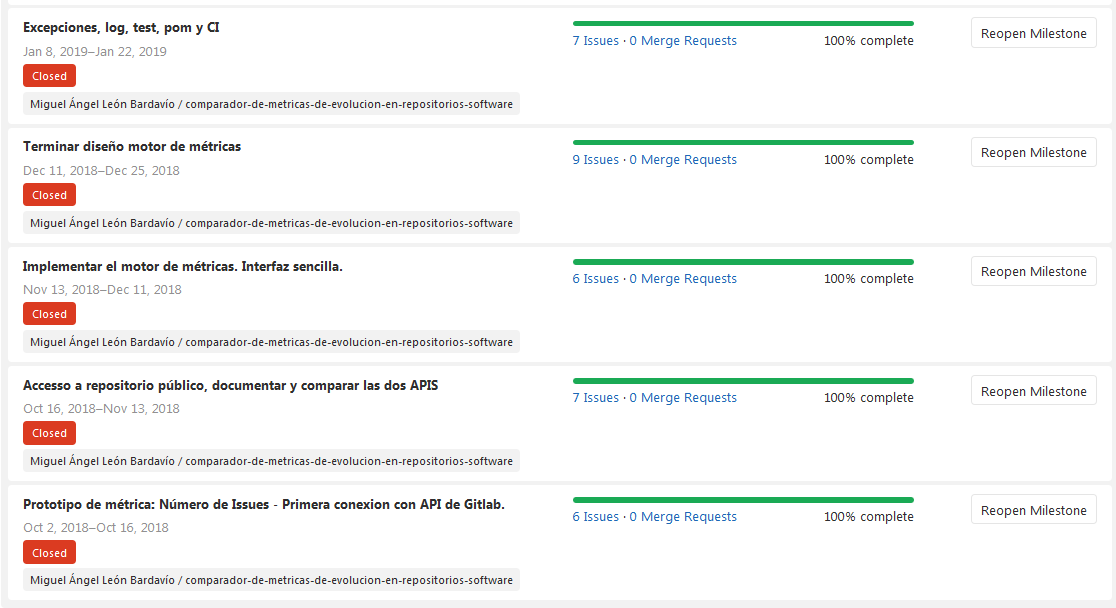
\includegraphics[scale=0.45]{Mgitlabmilestone.png}
	\caption{Milestone iniciales del proyecto en GitLab.}
	\label{fig:Mgitlabmilestone}
\end{figure}

\section{Documentación}
La fase de documentación duró un mes y fue a la par con la etapa de configuración. 

Se recopiló información sobre trabajos relacionados como \textit{Activiti-Api}\cite{rlp0019_software_2019}, \textit{Soporte de Métricas con Independencia del Lenguaje para la Inferencia de Refactorizaciones} \cite{marticorena_soporte_2005} y \textit{sPACE: Software Project Assessment in the Course of Evolution} \cite{ratzinger_space:_2007} y se estudió en qué entornos y qué herramientas se utilizarían para el desarrollo del proyecto.

Uno de los estudios más relevantes fue la elección de un API Java que permitiese la conexión a GitLab. Había tres opciones:
\begin{itemize}
	\item Crear un framework propio de conexión a GitLab a partir de GitLab API. Añadía cierta complejidad al proyecto al tener que desarrollar otro módulo más, pero permitía poder definir las funciones que se necesitaban.
	\item Usar timols/java-gitlab-api\footnote{\url{https://github.com/timols/java-gitlab-api}}\cite{olshansky_wrapper_2019}. Al principio fue la solución que se escogió, pero posteriormente se descubrió otro API bastante mejor. La documentación es bastante pobre y la evolución del proyecto software estaba parada o no evolucionaba bien, tenían demasiadas incidencias abiertas y no ofrecía gran parte de la funcionalidad que aportaba GitLab API.
	\item  Usar \footnote{\url{https://github.com/gitlab4j/gitlab4j-api}}\cite{noauthor_gitlab4j_2019}. Es un proyecto bastante decente y, a día de hoy, sigue creciendo. Tiene un alto porcentaje de incidencias cerradas, un gran número de releases, y evolución constante. Este es el API con el que se ha desarrollado este proyecto.
\end{itemize}
Otro de las decisiones más difíciles fue la versión de Java. Recientemente se lanzó la versión de Java 11 y es la que inicialmente se utilizó en el proyecto. Ha habido bastantes problemas de compatibilidad, pero se han ido solucionando a lo largo del tiempo.
\section{Configuración del flujo de trabajo del desarrollo software}
\subsection{Compilación y empaquetado}

El proyecto se iba a desarrollar en Java desde el principio, era un requisito no funcional. La versión más moderna que había cuando se comenzó el proyecto era Java 11. La decisión de utilizar esta versión de Java generó muchos problemas de compatibilidad de versiones con  otras bibliotecas en el desarrollo. 
\todo Enumerar cuales tenián problemas ¿ Vaadin?

En el proyecto se ha utilizado alguna de las nuevas versiones de Java no vista durante los curso. En el siguiente fragmento de código se describe 
un ejemplo de código que obtiene una colección de repositorios del usuario actual.
\tiny{
\begin{lstlisting}
...
if (connectionType != EnumConnectionType.NOT_CONNECTED) {
   return gitLabApi.getProjectApi().getUserProjectsStream(
   			currentUser.getId(),
   			new ProjectFilter())
		.map(p -> 
			new Repository(p.getWebUrl(), p.getName(), p.getId()))
		.collect(Collectors.toList());
			}
...
\end{lstlisting}
}

\section{Automatización de tareas de desarrollo}
\todo Describir el uso de Maven Ventajas e incovenientes
\subsection{Pruebas}
Para las pruebas se disponían de datos de otros repositorios de GitLab que se han presentado como TFG en el Grado de Ingeniería Informática en la 
Universidad de Burgos. Esto ha facilitado en gran medida el trabajo de pruebas. 
Es destacable la funcionalidad de acceso a los repositorios por el concepto de grupo definido en Gitlab. Esto fue posible gracias a que la empresa Hewlett Packard SCDS en su colabaración con TFG con la UBU organiza su propuestas de TFG en GitLab en grupos para organizarlos por cursos académicos.



Otro aspecto destacable es la uso con funciones avanzadas en la implementación de test unitarios. 
Como ejemplo en el siguiente fragmento de código se recoge como parametrizar un test para especificar un ficheros que recojan los múltiples casos de prueba.
De esta forma se simplifica mucho las prueba.

\todo se puede formatear mejor el código 
\tiny{
\begin{lstlisting}

@ParameterizedTest(name = "Run with User = \"{0}\" and 
	Password = \"{1}\" must throw an exception.")
@CsvFileSource(resources = "/testConnectUserPasswordWrong.csv", 
	numLinesToSkip = 1, delimiter = ';', encoding = "UTF-8")
						
public void testConnectUserPasswordWrong(String user, String password){
	assertThrows(RepositoryDataSourceException.class, () -> {
		repositoryDataSource.connect(user, password);},
		getErrorMsg("testConnectUserPasswordWrong", 
		"Wrong user-password should throw an exception"));
	assertEquals(EnumConnectionType.NOT_CONNECTED, 
		repositoryDataSource.getConnectionType(),
		getErrorMsg("testConnectUserPasswordWrong", 
		"Connection type must be 'NOT_CONNECTED'"));
}
\end{lstlisting}		

}

 

\subsection{Calidad continua}
En los últimos sprints, correspondientes a la entrega de prototipos funcionales al tutor,
se definía una tarea para analizar la deuda técnica que indicaba la Codacy.
Se analizaban las tareas de mejoras propuesta por Codacy según su orden de prioridad y se intentaban eliminar.
De esta forma además de aprender de las revisiones automáticas de Codacy se controlaba la deuda técnica, en el prototipo evolutivo.
La valoración final del proyecto ha sido la máxima (A) sin ninguna revivión de calidad de alta prioridad.
\todo Añadir url de codacy de tu proyecto y una captura de pantalla donde aparezca la A.

\subsection{Integración y despliegue continuo CI/CD}
Se han utilizado los sistemas de integración continua y despliegue continuo de GitLab para controlar el correcto funcionamiento de la aplicación después de un cambio y para mejorar la calidad de las revisiones.
La integración continua se ha configurado para que cada vez que se realiza un coomit en la rama principal del repositorio se compruebe que compila correctamente, que se ejecutan los test configurados en maven y se empaquete la aplicación Web en fichero war y se despligue en Heroku. Si alguna tarea falla se indica en el repositorio con un icono redondo rojo con aspa blanca.
\todo añadir una captura de pantalla con el badge Heroku del  Readme de Gitlab y explicar como se actualiza cada vez que se realiza un commit. 
\todo añadir una captura de pantalla con los check verdes en la lista de commit del repositorio de GitLab
